%% Default Latex document template
%%
%%  blake@rcs.ee.washington.edu

\documentclass[letterpaper]{article}

% Uncomment for bibliog.
%\bibliographystyle{unsrt}

\usepackage{graphicx}
\usepackage{lineno}
%\usepackage{fancyhdr}
\usepackage{tikz}
\usetikzlibrary{arrows.meta, positioning}
\begin{document}
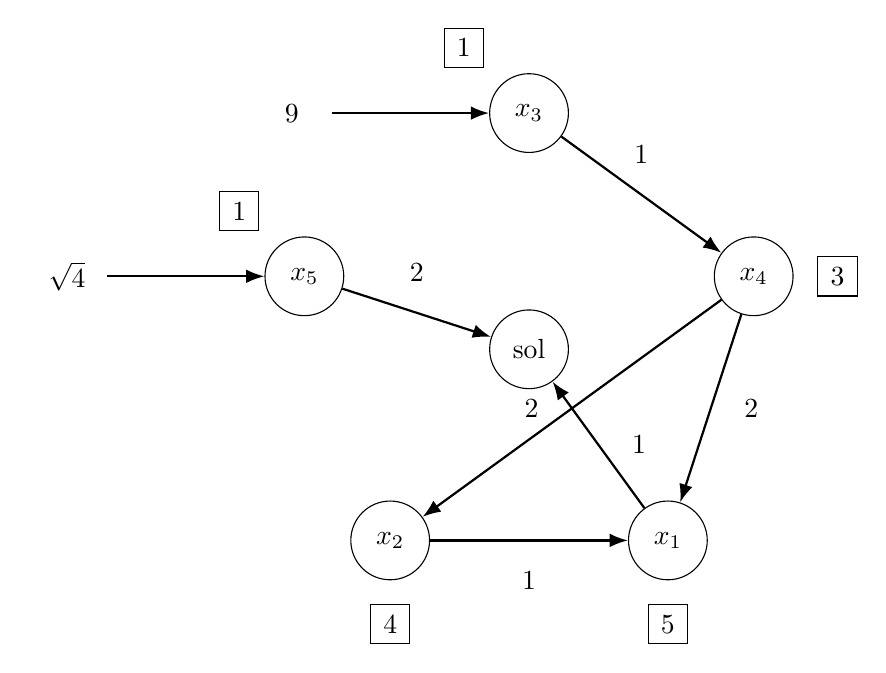
\begin{tikzpicture}[
    node distance=2cm,
    every node/.style={draw, circle, minimum size=1cm},
    label style/.style={draw=none, fill=none},
    every edge/.style={draw, -{Latex}, thick}
]

% Nodes arranged in a circle
\node (x3) at (90:3cm) {$x_3$};
\node (x4) at (18:3cm) {$x_4$};
\node (x1) at (306:3cm) {$x_1$};
\node (x2) at (234:3cm) {$x_2$};
\node (x5) at (162:3cm) {$x_5$};
% \node (sol) [right=1.75cm of x5] {sol};
\node (sol) at (0:0cm) {sol};

% Square annotations
\node[draw, rectangle, minimum size=0.5cm, below=3mm of x1] {5};
\node[draw, rectangle, minimum size=0.5cm, below=3mm of x2] {4};
\node[draw, rectangle, minimum size=0.5cm, above left=3mm of x3] {1};
\node[draw, rectangle, minimum size=0.5cm, right=3mm of x4] {3};
\node[draw, rectangle, minimum size=0.5cm, above left=3mm of x5] {1};


% Edges
\path (x3) edge node[label style, above] {1} (x4);
\path (x4) edge node[label style, left] {2} (x2);
\path (x4) edge node[label style, right] {2} (x1);
\path (x2) edge node[label style, below] {1} (x1);
\path (x5) edge node[label style, above] {2} (sol);
\path (x1) edge node[label style, right] {1} (sol);


% Input edges
\node (sqrt4) [left=of x5, draw=none] {$\sqrt{4}$};
\path (sqrt4) edge (x5);
\node (nine) [left=of x3, draw=none] {9};
\path (nine) edge (x3);

\end{tikzpicture}
\end{document}

